% ma489_presentation.tex
\documentclass[12pt]{beamer}
\usepackage{multicol}
\usepackage{tikz}
\usepackage{tikz-qtree}
\usepackage{wasysym}

\usetheme{Warsaw}
\useoutertheme{infolines}
\beamertemplatenavigationsymbolsempty
\begin{document}

%titlepage info
\title[RK Methods with Trees]{Runge-Kutta Methods with Rooted Trees}
\subtitle[motivation of project]{The Motivation of the Project}
\author[R. Douglas]{Richard Douglas}
\institute[WLU MA489]{
  MA489 Research Seminar at Wilfrid Laurier University
}
\date[November 2013]{November 12, 2013}

%for when I arrive at a new section
\AtBeginSection[]{
  \begin{frame}
    \frametitle{Outline}
    \tableofcontents[currentsection]
  \end{frame}
}

\begin{frame}
  \titlepage
\end{frame}

\section[Review of Numerical Methods]{A Brief Review of Numerical Methods for ODEs}
\begin{frame}{A brief review of numerical methods for ODEs}
  \begin{figure}
    \centering
    \includegraphics[width = \textwidth, height = 0.125\textheight]{./"images/subintervals"}
  \end{figure}
  Given an Ordinary Differential Equation of form
  $$y'(x) = f(x,y),  \forall x \in [a,b]$$
  with initial condition $y(a) = y_0$, \pause
  we can obtain a numerical approximation for $y(b)$ by first dividing the interval $[a,b]$ into $N$   
  equally spaced subintervals $[x_0,x_1], [x_1,x_2], ..., [x_{N-1},x_N]$ where
  $$h = \frac{(b - a)}{N}$$
  $$x_{n+1} = x_n + h$$
\end{frame}

\begin{frame}{Looking at individual steps}
  We then compute a sequence of approximations for $y(x)$ 
  $$y_0 = y(x_0), y_1 \approx y(x_1) = y(x_0 + h), \dots, y_N \approx y(x_N) = y(b)$$
  where the last value ends up being an approximation for $y$ when $x$ is at the end of the  
  interval. \newline
  \newline
  \pause
  We already know the value of $y_0$, \pause and $y_{n+1}$ can be obtained using its preceding 
  $y$ approximation.
  \pause
  $$y(a) = y_0 \to y_1\to \dots \to y_N \approx y(b)$$
\end{frame}

\begin{frame}{Example: Euler's method}
  $$x_{n+1} - x_n = h$$
  $$y_{n+1} = y_n + hf(x_n,y_n)$$
  \begin{figure}
    \centering
    \includegraphics[width = 0.65\textwidth, height = 0.65\textheight]{./"images/euler_method"}
  \end{figure}
\end{frame}

\begin{frame}{The order of a method}
  As the stepsize $h$ decreases, the numerical algorithm produces a better approximation for 
  $y(b)$. \newline
  \newline
  \pause
  That is to say
  $$\lim_{h \to 0} y_N = y(b)$$
  \pause
  We say that a method of approximation is of \textbf{order p} if
  $$\lim_{h \to 0} \frac{|y(b) - y_N|}{h^p} < \infty$$ \pause
  More compactly, we say that the method is $\mathbf{O(h^p)}$. \newline
  \newline
  \pause
  The order of a method tells us how fast it converges to the true value of 
  what it is approximating.
\end{frame}

\begin{frame}{Taylor methods}
  The usual way in which we derive a Runge-Kutta method of a given order is by comparing its   
  terms with a Taylor method of this order.
  \newline
  \newline
  \pause
  Taylor methods work using the Taylor Series expansion
  $$y(x) = y(x_n) + y'(x_n)(x - x_n) + \frac{y''(x_n)(x - x_n)^2}{2!} + \frac{y'''(x_n)(x - x_n)^3}{3!} + ...$$
  \pause
  So for an ODE with $y'(x) = f(x,y)$ and $y_0 = y(x_0)$, we will have
  \pause
  $$x_{n+1} - x_n = h$$
  \pause
  $$y_{n+1} = y_n + f(x_n,y_n)h + \frac{f'(x_n,y_n)h^2}{2!} + ... + \frac{f^{(p-1)}(x_n,y_n)h^p}{p!}$$
\end{frame}

\begin{frame}{The order of Taylor methods}
  For a Taylor method with
  $$y_{n+1} = y_n + f(x_n,y_n)h + \frac{f'(x_n,y_n)h^2}{2!} + ... + \frac{f^{(p-1)}(x_n,y_n)h^p}{p!}$$
  \pause
  The error in making a single step is $O(h^{p+1})$ and the error made across the entire interval 
   is $O(h^p)$. \newline
   \newline
   \pause
   What's nice about this is that if we want our numerical algorithm to be of a given order, then 
   there exists a Taylor method with that order. 
\end{frame}

\begin{frame}{The problem with Taylor methods}
  The main problem with Taylor methods is that we need to have the derivatives of $f(x,y)$.
  Assuming that they exist, differentiation grows more and more complicated as we take higher    
  derivatives.
  \pause
  $$f'(x,y) = f_x(x,y) + f_y(x,y)f(x,y)$$
  \pause
  $$f''(x,y) = f_{xx} + 2f_{xy}f + f_yf_x + f_{yy}f^2 + f_y^2f$$
  \pause
  $$f'''(x,y) = f_{xxx} + 3f_{xxy}f + 3f_{xyy}f^2 + f_{yyy}f^3 + $$
  $$f_y(f_{xx} + 2f_{xy}f + f_{yy}f^2) +  3(f_x + f_yf)(f_{xy} + f_{yy}f) + f_y^2(f_x + f_yf)$$
\end{frame}

\section[Runge-Kutta Definition]{Definition of Runge-Kutta Methods}
\begin{frame}{Runge-Kutta methods}
  Runge-Kutta methods on the other hand are much easier to code into a computer since once 
  you know the values of the parameters for a given Runge-Kutta method, the algorithm only 
  needs to compute values of $f$ during any given step. \newline
  \newline
  \pause
  Runge-Kutta methods work as follows: \newline
  \newline
  \pause
  Suppose that we have an ODE with
  $$y'(x) = f(x,y)$$
  $$\mbox{where } y_0 = y(x_0) \mbox{ is known}$$
  \pause
  As before, we will split the interval into subintervals of equal width $h$ and compute
  approximations $y_n$.
\end{frame}

\begin{frame}{How to do Runge-Kutta}
  To compute $y_{n+1}$, we compute approximations for $y$ for some choices
  of $x$ in the interval $[x_n,x_{n+1}]$. These approximations are called 
  \textbf{stages}. \newline
  \newline
  \pause
  The stages and their corresponding $x$ values are then plugged into $f(x,y)$ to obtain the
  \textbf{stage derivatives}. \newline
  \newline
  \pause
  So when going from $y_n$ to $y_{n+1}$ we will have $\mathbf{Y_1, Y_2, ..., Y_s}$ 
  as our stages and $\mathbf{f(X_1,Y_1), f(X_2,Y_2), ..., f(X_s,Y_s)}$ as our stage 
  derivatives.
\end{frame}

\begin{frame}{Computing stages}
  The first stage values in a step are $Y_1 = y_n$ and $f(X_1,Y_1) = f(x_n,y_n)$ \newline
  \newline
  \pause
  For explicit Runge-Kutta methods, the value of a stage is found by using the values of
  the stage derivatives of its preceding stages.
  \pause
  \begin{flalign*}
  Y_2 &= y_n + a_{21}hf(x_n,y_n) &\\ 
  &\\
  Y_3 &= y_n + a_{31}hf(X_1,Y_1) + a_{32}hf(X_2,Y_2) &\\
  &\\
  \vdots &\\
  Y_s &= y_n + \sum_{j=1}^{s-1}{a_{sj}hf(X_j,Y_j)} 
  \end{flalign*}
\end{frame}

\begin{frame}{Computing $y_{n+1}$}
  With the stages and stage derivatives now known, we obtain $y_{n+1}$ as $y_n$ plus a 
   weighted sum of the stage derivatives.
  \pause
  $$y_{n+1} = y_n + h\sum_{i = 1}^s{b_if(X_i,Y_i)}$$  
  \pause
  $$y_{n+1} = y_n + hb_1f(X_1,Y_1) + hb_2f(X_2,Y_2) + \dots + hb_sf(X_s,Y_s)$$
  \newline
  \pause
  The $b_i$ terms are known as the \textbf{weights}.
\end{frame}

\begin{frame}{X values}
  Recalling that 
  $$h = x_{n+1} - x_n$$
  \pause
  To be in the interval $[x_n,x_{n+1}]$, the $X_i$ values must be of form
  $$X_i = x_n + c_ih$$ 
  where the $c_i$ are in $[0,1]$. \newline
  \newline
  \pause
  Since $X_1 = x_n$, we have $c_1 = 0$
\end{frame}

\begin{frame}{Putting it all together}
  A convenient way to represent a Runge-Kutta method is by using a tableau of form
  \begin{table}
  \centering
  \renewcommand{\arraystretch}{1.25}
     \begin{tabular}{r | c*{4}{c}}
                        $0$ \\
                    $c_2$ & $a_{21}$ \\
                    $c_3$ & $a_{31}$ & $a_{32}$ \\
                   $\vdots$ & $\vdots$      &  $\vdots$  & $\ddots$ \\
	        $c_s$ & $a_{s1}$  &  $a_{s2}$  & $\dots$ & $a_{s(s-1)}$\\
                     \hline
    \phantom{c4}     & $b_1$ & $b_2$ & $\dots$ & $b_s$ \\
    \end{tabular}
  \renewcommand{\arraystretch}{1.0}
  \end{table}
  \pause
  Where
  \begin{itemize}
    \item $a_{ij}$ represents how stage $i$ depends on the $jth$ stage derivative,
    \item $b_i$ represents the weight of $hf(X_i,Y_i)$ in computing $y_{n+1}$,
    \item $c_i$ represents the location of $X_i$ in the interval $[x_n,x_{n+1}]$
  \end{itemize}
\end{frame}

\section[Deriving Runge-Kutta]{Deriving Runge-Kutta Methods}
\begin{frame}{Deriving Runge-Kutta methods}
  Now suppose that we want a Runge-Kutta method that has a global error of $O(h^p)$.
  How do we choose the values of the $a_{ij}$, the $b_i$, and the $c_i$? \newline
  \newline
  \pause
  This is where the Taylor methods come into play. \newline
  \newline
  \pause
  First we choose the number of stages to use in the algorithm. At least $s = p$ stages
  are necessary and there are advantages to using $s = p + 1$. \newline
  \newline
  \pause
  Then we compute the Taylor series expansions for the Taylor method of order $p$ and
  the Runge-Kutta method with $s$ stages. Equating coefficients leads us to a system of
  equations which when solved, tells us the values we can use for the Runge-Kutta method's
  parameters.
\end{frame}

\begin{frame}{A necessary tool for deriving Runge-Kutta methods}
  In order to compare the Taylor series expansions we need the following general result:
  \begin{theorem}{\textbf{Bivariate Taylor Expansion:}}
    Let $f(x,y)$ be an infinitely differentiable function in some open neighbourhood around
    $(x_0,y_0)$, then
    $$f(x,y) = f(x_0,y_0) + f_x(x-x_0) + f_y(y-y_0) $$
    \pause
    $$+\frac{1}{2!}(f_{xx}(x-x_0)^2 + f_{xy}(x-x_0)(y-y_0)$$
    $$+ f_{yx}(y-y_0)(x-x_0) + f_{yy}(y-y_0)^2)$$
    $$+ \dots$$
  \end{theorem}
\end{frame}

\begin{frame}{2nd order Runge-Kutta methods with 2 stages}
  These methods have X values
  $$X_1 = x_n, X_2 = x_n + c_2h,$$
  \pause
  stages
  $$Y_1 = y_n, Y_2 = y_n + a_{21}hf(x_n,y_n),$$
  \pause
  and stage derivatives
  $$f(X_1,Y_1) = f(x_n,y_n),$$ 
  $$f(X_2,Y_2) = f(x_n + c_2h, y_n + a_{21}hf(x_n,y_n)).$$
\end{frame}

\begin{frame}{Obtaining the Taylor expansions}
  We thus have
  $$y_{n+1} = y_n + hb_1f(x_n,y_n) + hb_2f(x_n + c_2h,y_n + a_{21}hf(x_n,y_n))$$
  \pause
  with expansion
  $$y(x_{n+1}) = y_n + b_1hf + b_2hf + b_2c_2h^2f_x + b_2a_{21}h^2f_yf + O(h^3)$$
  \pause
  The Taylor method of order 2 is 
  $$y_{n+1} = y_n + f(x_n,y_n)h + \frac{f'(x_n,y_n)h^2}{2!}$$
  \pause
  with simplified expansion
  $$y(x_{n+1}) = y_n + hf + \frac{h^2f_x}{2} + \frac{h^2f_yf}{2} + O(h^3)$$
\end{frame}

\begin{frame}{Comparing the Taylor expansions}
  $$y(x_{n+1}) = y_n + b_1hf + b_2hf + b_2c_2h^2f_x + b_2a_{21}h^2f_yf + O(h^3)$$
  $$y(x_{n+1}) = y_n + hf + \frac{h^2f_x}{2} + \frac{h^2f_yf}{2} + O(h^3)$$
  \pause
  Equating coefficients gives us the system of equations
  $$b_1 + b_2 = 1$$
  $$b_2c_2 = \frac{1}{2}$$
  $$b_2a_{21} = \frac{1}{2}$$
\end{frame}

\begin{frame}{Obtaining the parameter values}
  Allowing $b_2$ to be a free parameter gives us the solution
  $$b_1 = 1 - b_2$$
  $$c_2 = \frac{1}{2b_2}$$
  $$a_{21} = \frac{1}{2b_2}$$
  \pause
  So all 2nd order Runge-Kutta methods with two stages are of form
  \begin{table}
  \centering
  \renewcommand{\arraystretch}{1.25}
     \begin{tabular}{r | c*{2}{c}}
                        $0$ \\
                    $\frac{1}{2b_2}$ & $\frac{1}{2b_2}$ \\
                     \hline
    \phantom{c4}     & $1 - b_2$ & $b_2$
    \end{tabular}
  \renewcommand{\arraystretch}{1.0}
  \end{table}
\end{frame}

\begin{frame}{Special cases of 2nd order Runge-Kutta methods}
  \begin{table}
  \centering
  \renewcommand{\arraystretch}{1.25}
     \begin{tabular}{r | c*{2}{c}}
                        $0$ \\
                    $\frac{1}{2b_2}$ & $\frac{1}{2b_2}$ \\
                     \hline
    \phantom{c4}     & $1 - b_2$ & $b_2$
    \end{tabular}
  \renewcommand{\arraystretch}{1.0}
  \end{table}
  \pause
  Setting $b_2 = 1$ gives us the \textbf{midpoint method}
  $$y_{n+1} = y_n + hf(x_n + \frac{h}{2}, y_n + \frac{h}{2}f(x_n,y_n))$$
  \pause
  and setting $b_2 = \frac{1}{2}$ gives us \textbf{Heun's method}.
  $$y_{n+1} = y_n + \frac{h}{2}f(x_n,y_n) + \frac{h}{2}f(x_n + h, y_n + hf(x_n,y_n))$$
\end{frame}

\begin{frame}{The RK4}
  One of the most popular Runge-Kutta methods used in practice is the RK4.
  The RK4 is a fourth order method with 4 stage values. It achieves a nice balance
  of being precise and not requiring a lot of stage value computations. \newline
  \newline
  \pause
  The RK4 is as follows
  \pause
  $$f(X_1,Y_1) = f(x_n,y_n)$$
  $$f(X_2,Y_2) = f(x_n + \frac{h}{2}, y_n + \frac{h}{2}f(X_1,Y_1))$$
  $$f(X_3,Y_3) = f(x_n + \frac{h}{2}, y_n + \frac{h}{2}f(X_2,Y_2))$$
  $$f(X_4,Y_4) = f(x_n + h, y_n + hf(X_3,Y_3))$$
\end{frame}

\begin{frame}{The RK4 (continued)}
  with weights
  $$y_{n+1} = y_n + \frac{h}{6}f(X_1,Y_1) + \frac{h}{3}f(X_2,Y_2) + 
  \frac{h}{3}f(X_3,Y_3) + \frac{h}{6}f(X_4,Y_4)$$
  \pause
  and tableau \newline

  \begin{table}
  \centering
  \renewcommand{\arraystretch}{1.25}
     \begin{tabular}{r | c*{4}{c}}
                        $0$ \\
        $\frac{1}{2}$ & $\frac{1}{2}$ \\
        $\frac{1}{2}$ &          $0$         & $\frac{1}{2}$ \\
                        $1$ &          $0$         &           $0$        & $1$ \\
                     \hline
    \phantom{c4}     & $\frac{1}{6}$ & $\frac{1}{3}$ & $\frac{1}{3}$ & $\frac{1}{6}$ \\
    \end{tabular}
  \renewcommand{\arraystretch}{1.0}
  \end{table}
\end{frame}

\begin{frame}{The problem with higher order Runge-Kutta methods}
  In practice, higher order Runge-Kutta methods may not be as attractive as the RK4 as they
  require more stage values and stage derivatives to be computed. \newline
  \newline
  \pause
  Another more interesting problem is that as the required order increases
  when we are deriving Runge-Kutta methods,
  \begin{itemize}
    \pause
    \item we need higher derivatives of $f(x,y)$ for the coefficients of the Taylor method,
    \pause
    \item we will need more terms from the bivariate Taylor expansion,
    \pause
    \item more stage derivatives are popping up in the computation of $Y_i$. 
  \end{itemize}
\end{frame}

\begin{frame}{System of equations for 4th order methods with four stages}
  $$a_{21} = c_2$$
  $$a_{31} + a_{32} = c_3$$
  $$a_{41} + a_{42} + a_{43} = c_4$$
  $$b_1 + b_2 + b_3 + b_4 = 1$$
  $$b_2c_2 + b_3c_3 + b_4c_4 = \frac{1}{2}$$
  $$b_2c_2^2 + b_3c_3^2 + b_4c_4^2 = \frac{1}{3}$$
  $$b_2c_2^3 + b_3c_3^3 + b_4c_4^3 = \frac{1}{4}$$
\end{frame}

\begin{frame}{System of equations for 4th order methods with four stages (continued)}
  $$b_3a_{32}c_2 + b_4a_{42}c_2 + b_4a_{43}c_3 = \frac{1}{6}$$
  $$b_3c_3c_2a_{32} + b_4c_4c_2a_{42} + b_4c_4c_3a_{43} = \frac{1}{8}$$
  $$b_3c_2^2a_{32} + b_4c_2^2a_{42} + b_4c_3^2a_{43} = \frac{1}{12}$$
  $$b_4c_2a_{32}a_{43} = \frac{1}{24}$$
  \pause
  From the way these equations are written, we can see some patterns.
\end{frame}

\section[Project Goal]{The Goal of the Project}
\begin{frame}{The goal of the project}
  If we know the system of equations that the parameters need to satisfy,
  then we don't need to do any Taylor expansions or take any derivatives of $f$. \newline
  \newline
  \pause
  Solving the system tells us how to program Runge-Kutta methods into the computer. \newline
  \newline
  \pause
  How else can we obtain the system of equations? \newline
  \newline
  \pause
  What is the pattern?
\end{frame}

\begin{frame}{The pattern} 
  The first 3 equations
  $$a_{21} = c_2$$
  $$a_{31} + a_{32} = c_3$$
  $$a_{41} + a_{42} + a_{43} = c_4$$
  Correspond to summing the rows of $a$'s in order to get the $c$ values
  \begin{table}
  \centering
  \renewcommand{\arraystretch}{1.25}
     \begin{tabular}{r | c*{4}{c}}
                        $0$ \\
                    $c_2$ & $a_{21}$ \\
                    $c_3$ & $a_{31}$ & $a_{32}$ \\
	        $c_4$ &  $a_{41}$  &  $a_{42}$  & $a_{43}$\\
                     \hline
    \phantom{c4}     & $b_1$ & $b_2$ & $b_3$ & $b_4$ \\
    \end{tabular}
  \renewcommand{\arraystretch}{1.0}
  \end{table}
\end{frame}

\begin{frame}{Equations with trees}
  \begin{multicols}{2}
  \begin{tikzpicture}
     \tikzset{grow'=up}
     \Tree [ .$o$ ]
  \end{tikzpicture}
  \vfill
   \begin{tikzpicture}
    \tikzset{grow'=up}
    \Tree [.$o$ [.$o$ ] ] ]
  \end{tikzpicture}
  \vfill
  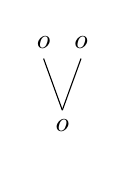
\begin{tikzpicture}
    \tikzset{grow'=up}
    \Tree [.$o$ [.$o$ ] [.$o$ ] ] ]
  \end{tikzpicture}
  \vfill
  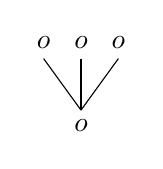
\begin{tikzpicture}
    \tikzset{grow'=up}
    \Tree [.$o$ [.$o$ ] [.$o$ ] [.$o$ ] ] ]
  \end{tikzpicture}
  \vfill
  \columnbreak

  $$b_1 + b_2 + b_3 + b_4 = 1$$
  \vfill
  $$b_1c_1 + b_2c_2 + b_3c_3 + b_4c_4 = \frac{1}{2}$$
  \vfill
  $$b_1c_1^2 + b_2c_2^2 + b_3c_3^2 + b_4c_4^2 = \frac{1}{3}$$ 
  \vfill
  $$b_1c_1^3 + b_2c_2^3 + b_3c_3^3 + b_4c_4^3 = \frac{1}{4}$$  
  \vfill
  \end{multicols}
\end{frame}

\begin{frame}{Equations with trees (continued)}
  \begin{multicols}{2}
  \begin{tikzpicture}
   \centering 
   \tikzset{grow'=up}
    \Tree [.$o$ [.$o$ $o$ ] ]
  \end{tikzpicture}
  \vfill
  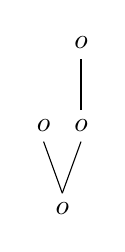
\begin{tikzpicture}
   \centering 
   \tikzset{grow'=up}
    \Tree [.$o$ [.$o$ ]  [.$o$ $o$ ]]
  \end{tikzpicture}
  \vfill
  
  \columnbreak
  $$\sum_{i, j=1}^s{b_ia_{ij}c_j} = \frac{1}{6}$$
  \vfill
  $$\sum_{i, j=1}^s{b_ic_ia_{ij}c_j} = \frac{1}{8}$$
  \vfill
  \end{multicols}
\end{frame}

\begin{frame}{Equations with trees (continued)}
  \begin{multicols}{2}
   \begin{tikzpicture}
   \tikzset{grow'=up}
    \Tree [.$o$ [.$o$ [.$o$ [ .$o$ ] ] ] ]
  \end{tikzpicture}
  \vfill
  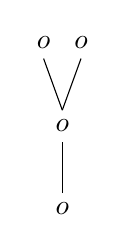
\begin{tikzpicture}
   \tikzset{grow'=up}
    \Tree [.$o$ [.$o$ $o$ $o$ ] ]
  \end{tikzpicture}
  \vfill
  \columnbreak
   $$\sum_{i, j, k=1}^s{b_ia_{ij}a_{jk}c_k} = \frac{1}{24}$$
  \vfill
  $$\sum_{i, j=1}^s{b_ia_{ij}c_j^2} = \frac{1}{12}$$
  \vfill
  \end{multicols}
\end{frame}

\begin{frame}{Obtaining the trees}
  \pause
  First order \newline
  \newline
  \begin{tikzpicture}
     \tikzset{grow'=up}
     \Tree [ .$o$ ]
  \end{tikzpicture}

  \pause
  Second order \newline
  \newline
  \begin{tikzpicture}
    \tikzset{grow'=up}
    \Tree [.$o$ [.$o$ ] ] ]
  \end{tikzpicture}

  \pause
  Third order \newline
  \newline
   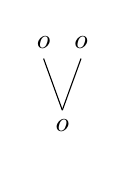
\begin{tikzpicture}
    \tikzset{grow'=up}
    \Tree [.$o$ [.$o$ ] [.$o$ ] ] ]
  \end{tikzpicture}
  \begin{tikzpicture}
   \tikzset{grow'=up}
    \Tree [.$o$ [.$o$ $o$ ] ]
  \end{tikzpicture}
\end{frame}

\begin{frame}{Fourth order trees}
  Fourth order \newline
  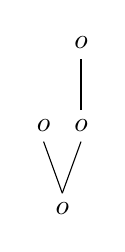
\begin{tikzpicture}
   \tikzset{grow'=up}
    \Tree [.$o$ [.$o$ ]  [.$o$ $o$ ]]
  \end{tikzpicture}
  \newline
  \begin{tikzpicture}
   \tikzset{grow'=up}
    \Tree [.$o$ [.$o$ [.$o$ [ .$o$ ] ] ] ]
  \end{tikzpicture}
  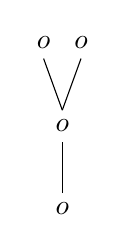
\begin{tikzpicture}
   \tikzset{grow'=up}
    \Tree [.$o$ [.$o$ $o$ $o$ ] ]
  \end{tikzpicture}
  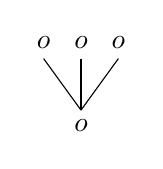
\begin{tikzpicture}
    \tikzset{grow'=up}
    \Tree [.$o$ [.$o$ ] [.$o$ ] [.$o$ ] ] ]
  \end{tikzpicture}
\end{frame}

\begin{frame}{Conclusion}
  The goal of the project is to understand (with proof) how to use rooted trees to
  derive the system of equations for Runge-Kutta methods of a given order. \newline
  \newline
  \pause
  I may also look at the group formed by these trees (also known as the \textbf{Butcher group}).
  \newline
  \newline
  \pause
  Thank you for viewing my presentation \smiley.
\end{frame}
 
\section*{References}
\begin{frame}{References}
Main reference
\begin{itemize} \item Butcher, John C., \textit{Numerical Methods for Ordinary Differential Equations} (2008), second edition \end{itemize}
Textbook references
\begin{itemize}
  \item Nagle et al., \textit{Fundamentals of Differential Equations and Boundary Value Problems}
           (2012), sections 3.6 and 3.7, sixth edition
  \item Matthews, John H. and Fink, Kurtis D., \textit{Numerical Methods using Matlab} (2004),
           sections 9.4 and 9.5, fourth edition 
\end{itemize}
Internet references

\begin{itemize}
  \item Kaw, Autar K., \textit{Numerical Methods with Applications},
          \textit{http://mathforcollege.com/nm/topics/textbook\_index.html}
  \item The Wikipedia page on Runge-Kutta methods, \textit{http://en.wikipedia.org/wiki/Runge-Kutta}
\end{itemize}

% Both sites visited most recently (at the time of writing) on Nov. 10, 2013.
\end{frame}

\end{document}